\chapter{Analisis Persoalan dan Rancangan Solusi}

Tujuan utama penulisan bab ini adalah untuk menguraikan rencana penyelesaian masalah tugas akhir sebelum dieksekusi. Bagian ini akan memaparkan proses analisis masalah hingga menjadi solusi.

\section{Analisis Persoalan}


\section{Analisis Solusi}

Terdapat dua masalah yang perlu diselesaikan dalam penyusunan solusi?

\begin{enumerate}
    \item Bagaimana efektivitas dari teknik PETL? Bagaimana perbandingannya?
\end{enumerate}

Masalah pertama berkaitan dengan mengevaluasi efektivitas teknik-teknik PETL dalam meningkatkan kinerja IndoBERT. Untuk ini, perlu dilakukan eksperimen yang komprehensif di mana setiap teknik PETL seperti LoRA, \textit{Prefix-Tuning}, dan \textit{Tiny-Attention Adapter} Adapter diuji dalam berbagai tugas NLP. Evaluasi ini akan mengukur peningkatan kinerja yang dicapai oleh setiap teknik, memberikan data empiris tentang efektivitas mereka.

Selain mengukur efektivitas masing-masing, penting juga untuk membandingkan kinerja antar teknik PETL. Analisis ini akan melibatkan pengujian setiap teknik dalam kondisi yang serupa, memastikan bahwa perbandingan kinerja mereka adil dan akurat. Ini akan membantu dalam mengidentifikasi teknik mana yang paling efektif dan di bawah kondisi apa.

\begin{enumerate}
    \item Bagaimana penggunaan sumber daya dari setiap teknik?
\end{enumerate}

Masalah kedua berkaitan dengan efisiensi penggunaan sumber daya oleh teknik PETL dibandingkan dengan fine-tuning tradisional. Ini melibatkan pengukuran waktu pelatihan, penggunaan memori, dan jumlah parameter yang diperbarui. Evaluasi ini penting untuk menentukan apakah teknik PETL benar-benar lebih efisien dalam hal sumber daya komputasi.

Untuk mengatasi masalah-masalah ini, penelitian ini akan menggunakan serangkaian eksperimen dan analisis untuk mengevaluasi dan membandingkan teknik PETL. Pendekatan ini akan memungkinkan penelitian untuk memberikan wawasan yang mendalam tentang efektivitas dan efisiensi berbagai teknik PETL dalam konteks IndoBERT, serta memberikan rekomendasi tentang pendekatan terbaik untuk meningkatkan kinerja model dalam berbagai tugas pemrosesan bahasa alami.


\subsection{Rencana Penanganan Masalah dan Analisis Kebutuhan}

\section{Rancangan Solusi}
\label{sec:rancangan-solusi}

Langkah umum untuk mencapai solusi masalah di Tugas Akhir ditunjukkan pada gambar \ref*{fig:langkah-umum} berikut.

\begin{figure}[ht]
    \centering
    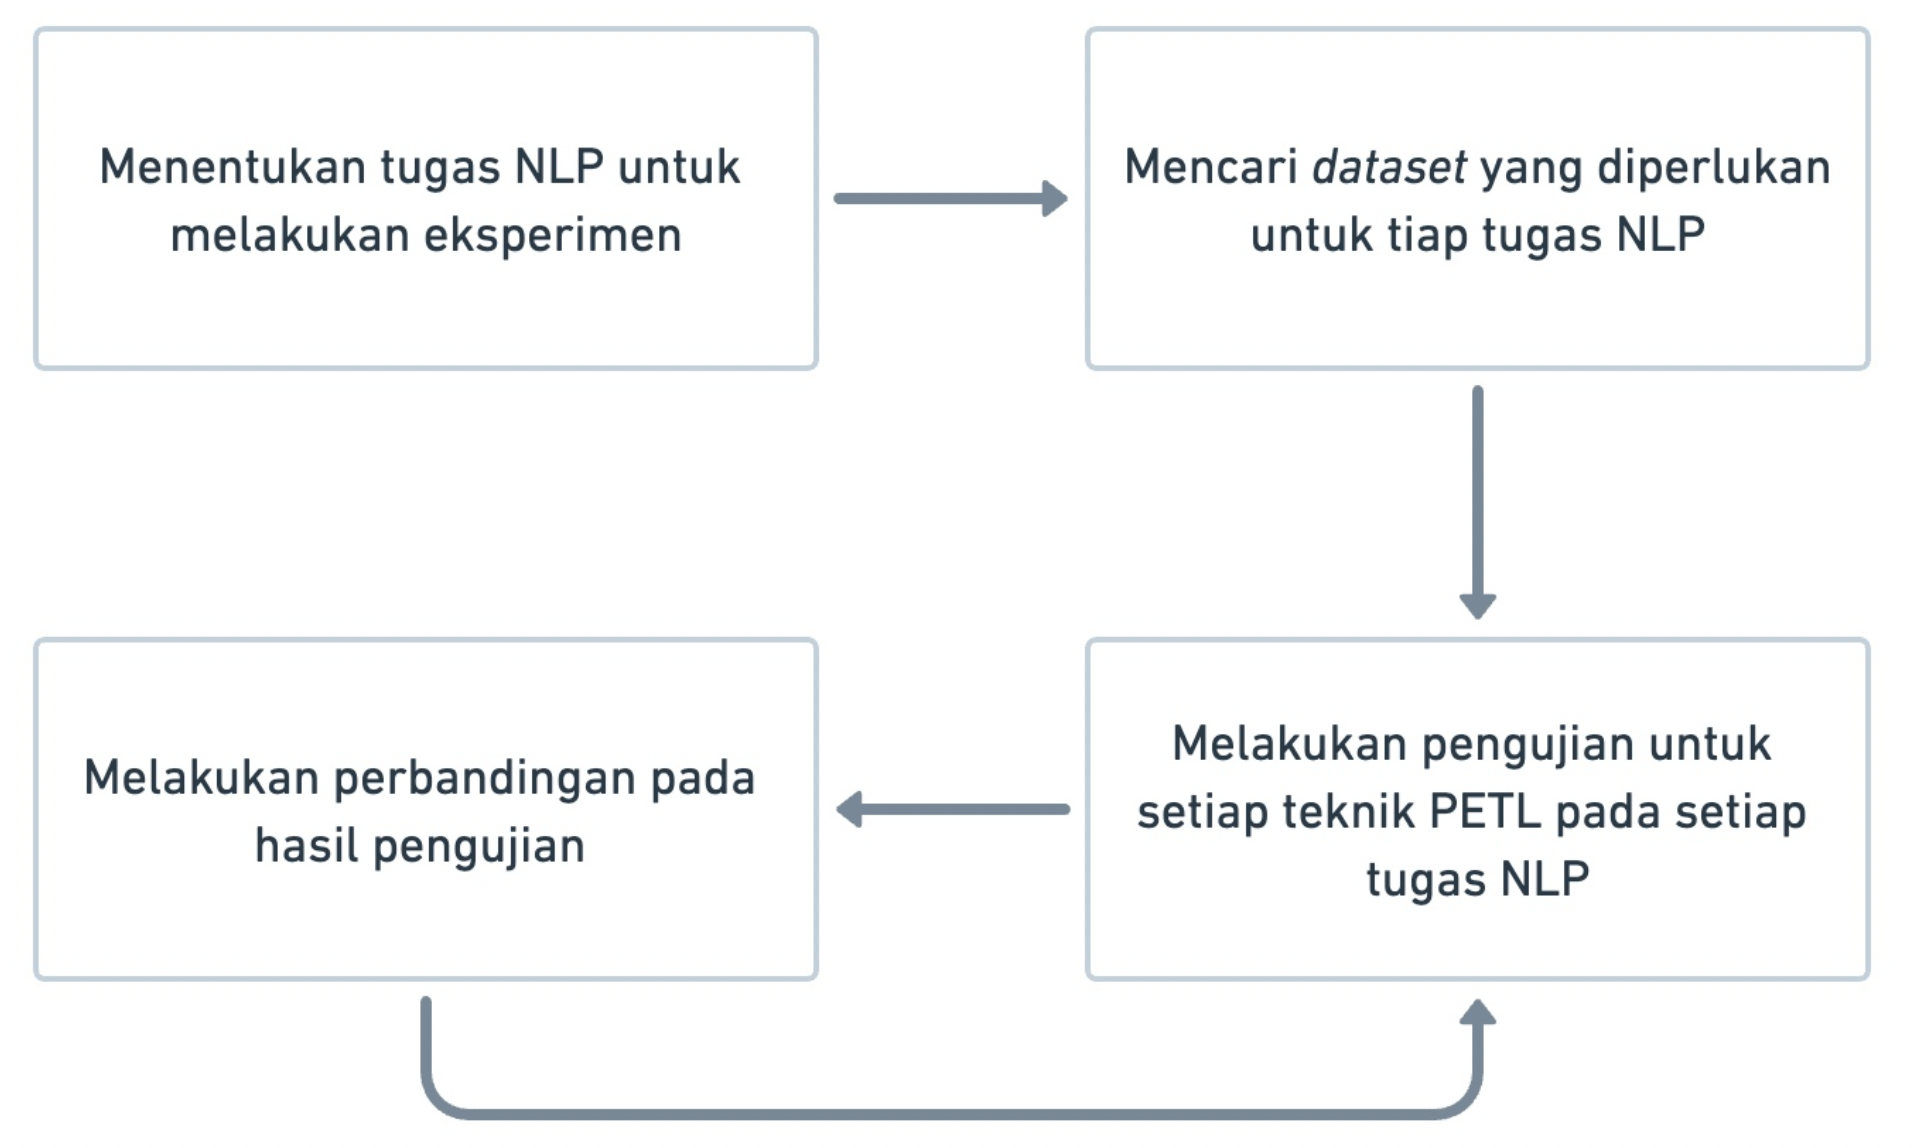
\includegraphics[width=0.8\textwidth]{chapter-3/langkah_umum.png}
    \caption{Langkah Umum Solusi}
    \label{fig:langkah-umum}
\end{figure}

Dataset yang diperlukan akan diambil dari \cite{nusacatalogue}. Teknik PETL yang digunakan adalah LoRA (\textit{Low-Rank Adaptation}), \textit{Prefix-Tuning}, dan \textit{Tiny-Attention Adapter}. Hasil pengujian berupa kinerja dari teknik PETL serta penggunaan sumber daya dari setiap eksperimen.